%Version 3.1 December 2024
% See section 11 of the User Manual for version history
%
%%%%%%%%%%%%%%%%%%%%%%%%%%%%%%%%%%%%%%%%%%%%%%%%%%%%%%%%%%%%%%%%%%%%%%
%%                                                                 %%
%% Please do not use \input{...} to include other tex files.       %%
%% Submit your LaTeX manuscript as one .tex document.              %%
%%                                                                 %%
%% All additional figures and files should be attached             %%
%% separately and not embedded in the \TeX\ document itself.       %%
%%                                                                 %%
%%%%%%%%%%%%%%%%%%%%%%%%%%%%%%%%%%%%%%%%%%%%%%%%%%%%%%%%%%%%%%%%%%%%%

%%\documentclass[referee,sn-basic]{sn-jnl}% referee option is meant for double line spacing

%%=======================================================%%
%% to print line numbers in the margin use lineno option %%
%%=======================================================%%

%%\documentclass[lineno,pdflatex,sn-basic]{sn-jnl}% Basic Springer Nature Reference Style/Chemistry Reference Style

%%=========================================================================================%%
%% the documentclass is set to pdflatex as default. You can delete it if not appropriate.  %%
%%=========================================================================================%%

%%\documentclass[sn-basic]{sn-jnl}% Basic Springer Nature Reference Style/Chemistry Reference Style

%%Note: the following reference styles support Namedate and Numbered referencing. By default the style follows the most common style. To switch between the options you can add or remove �Numbered� in the optional parenthesis. 
%%The option is available for: sn-basic.bst, sn-chicago.bst%  

%%\documentclass[pdflatex,sn-nature]{sn-jnl}% Style for submissions to Nature Portfolio journals
%%\documentclass[pdflatex,sn-basic]{sn-jnl}% Basic Springer Nature Reference Style/Chemistry Reference Style
\documentclass[pdflatex,sn-mathphys-num]{sn-jnl}% Math and Physical Sciences Numbered Reference Style
%%\documentclass[pdflatex,sn-mathphys-ay]{sn-jnl}% Math and Physical Sciences Author Year Reference Style
%%\documentclass[pdflatex,sn-aps]{sn-jnl}% American Physical Society (APS) Reference Style
%%\documentclass[pdflatex,sn-vancouver-num]{sn-jnl}% Vancouver Numbered Reference Style
%%\documentclass[pdflatex,sn-vancouver-ay]{sn-jnl}% Vancouver Author Year Reference Style
%%\documentclass[pdflatex,sn-apa]{sn-jnl}% APA Reference Style
%%\documentclass[pdflatex,sn-chicago]{sn-jnl}% Chicago-based Humanities Reference Style

%%%% Standard Packages
%%<additional latex packages if required can be included here>

\usepackage{graphicx}%
\usepackage{multirow}%
\usepackage{amsmath,amssymb,amsfonts}%
\usepackage{amsthm}%
\usepackage{mathrsfs}%
\usepackage[title]{appendix}%
\usepackage{xcolor}%
\usepackage{textcomp}%
\usepackage{manyfoot}%
\usepackage{booktabs}%
\usepackage{algorithm}%
\usepackage{algorithmicx}%
\usepackage{algpseudocode}%
\usepackage{listings}%
%%%%
\usepackage{adjustbox}
%\usepackage{booktabs}
\usepackage{longtable}

%%%%%=============================================================================%%%%
%%%%  Remarks: This template is provided to aid authors with the preparation
%%%%  of original research articles intended for submission to journals published 
%%%%  by Springer Nature. The guidance has been prepared in partnership with 
%%%%  production teams to conform to Springer Nature technical requirements. 
%%%%  Editorial and presentation requirements differ among journal portfolios and 
%%%%  research disciplines. You may find sections in this template are irrelevant 
%%%%  to your work and are empowered to omit any such section if allowed by the 
%%%%  journal you intend to submit to. The submission guidelines and policies 
%%%%  of the journal take precedence. A detailed User Manual is available in the 
%%%%  template package for technical guidance.
%%%%%=============================================================================%%%%

%% as per the requirement new theorem styles can be included as shown below
\theoremstyle{thmstyleone}%
\newtheorem{theorem}{Theorem}%  meant for continuous numbers
%%\newtheorem{theorem}{Theorem}[section]% meant for sectionwise numbers
%% optional argument [theorem] produces theorem numbering sequence instead of independent numbers for Proposition
\newtheorem{proposition}[theorem]{Proposition}% 
%%\newtheorem{proposition}{Proposition}% to get separate numbers for theorem and proposition etc.

\theoremstyle{thmstyletwo}%
\newtheorem{example}{Example}%
\newtheorem{remark}{Remark}%

\theoremstyle{thmstylethree}%
\newtheorem{definition}{Definition}%

\raggedbottom
%%\unnumbered% uncomment this for unnumbered level heads

\begin{document}
	
	\title[From gatekeeping to help-seeking: post-victimization behavior as a social process rather than a single decision to report]{From gatekeeping to help-seeking: post-victimization behavior as a social process rather than a single decision to report}
	
	%%=============================================================%%
	%% GivenName	-> \fnm{Joergen W.}
	%% Particle	-> \spfx{van der} -> surname prefix
	%% FamilyName	-> \sur{Ploeg}
	%% Suffix	-> \sfx{IV}
	%% \author*[1,2]{\fnm{Joergen W.} \spfx{van der} \sur{Ploeg} 
		%%  \sfx{IV}}\email{iauthor@gmail.com}
	%%=============================================================%%
	
	\author[1]{\fnm{Sergey} \sur{Bondarkov}}\email{sbondarkov@eu.spb.ru}
	
	
	\affil[1]{\orgdiv{The Institute for the Rule of Law}, \orgname{the European University at Saint Petersburg}, \orgaddress{\street{6/1~A~Gagarinskaya Street}, \city{St.~Petersburg}, \postcode{191187}, \country{Russia}}}
	
	
	%%==================================%%
	%% Sample for unstructured abstract %%
	%%==================================%%
	
	\abstract{\textbf{Purpose:} To reframe post-victimization behavior as help-seeking process, and establish covariates of basic victims' strategies operationalized as combinations of formal and informal sources of help used, i.e. reporting to the police and activating one's personal network.
		
		\textbf{Methods:} This paper uses the Russian Crime Victimization Survey (2018, 2021, 2024; 6,684 completed crime victims), which has the advantage of asking victims if they told friends or family about an incident --- a question that is absent from the most widely used victimization surveys. This enables me to explore associations between 1) sharing with friends or family and notifying the police, 2) situational, as well as a victim's socio-ecomonic characteristics and the probability of employing a certain help-seeking strategy. Such modeling is done separately for violent, property and cyber crime.
		
		\textbf{Results:} After controlling for crime gravity and other incident characteristics, I find that 1) informing friends or family is associated with increased probability that the law enforcement learns about a crime, 2) a victim's age, gender and, in cases of violent incident, relative distance to the offender predict which `pathway' they take in navigating post-victimization. Also, repeat victims and those blaming themselves are more likely to share with friends only or to remain silent. 
		
		\textbf{Conclusion:} Thinking about responding to victimization as an interactive social process offers new insights into what structures decisions to report a crime. At the same time, it highlights the deficiency of our current data and calls for revision of victimization survey instruments.}
	
	
	\keywords{victimization, reporting crime, help-seeking, social networks, RCVS}
	
	%%\pacs[JEL Classification]{D8, H51}
	
	%%\pacs[MSC Classification]{35A01, 65L10, 65L12, 65L20, 65L70}
	
	\maketitle
	
	\section*{Introduction}\label{intro}
	From the very beginning of research on reporting victimization there were indications of the interactive nature of the process. Two massive studies of police response time \citep{van1978response, spelman1985calling} found that most of the time dialing the police was `delayed' by people talking to others, either witnesses or advisors, in order to gather information, make sense of the situation or cope with stress. Yet, decades later, \citet{knoth2019reporting} still had to conclude that `studies that assess differences between individuals who report to the police, seek alternative help, or do nothing [...] often fail to recognize that individuals who do end up calling the police are likely to first seek advice from a third party'. Two recent reviews of the current knowledge on how decisions to report are made \citep{xie2019crime,bergemann2024social} both acknowledged lack of integrative models, accounting not only for incident gravity, the victim's socio-economic status, or their relative distance to the offender, but also for possible social influence. \citet{xie2019crime}
	also pointed to a simple explanation for this unlikely situation: the lack of data. Indeed, in the NCVS, a question about informing some party other than police first appeared only in the latest update, and the data gathered with the new instrument is yet to be published. In the CSEW such question is reserved for 10-15 year-olds only. The ICVS never featured such a question. How this came about is another interesting puzzle we will touch upon later\footnote{Incidentally, the similar sentiment is found in legal needs literature. Despite the evidence for importance of lay advice for contacting a lawyer with a legal problem \citep{ogp2019access} the discipline is said to be lagging behind medical literature which embraced social network perspective long ago \citep{buck2010community}. Importantly, the current data gathering instruments used in the field do not provide sufficient information on this aspect of the problem \citep{abf2025access}.}. Of more practical interest is where to find data that allow to test integrative frameworks in the spirit of those suggested by \citep{xie2019crime,bergemann2024social}.
	
	In this paper I use the Russian Crime Victimization Survey (RCVS) \citep{kuchakov2026rcvs}, a regular and nationally representative monitoring that targets Russian citizens of 18 years and older. The RCVS has the advantage of recording if a victim told their friends or family about the incident. Recent analysis by \citet{dzmitryieva2025crime} employing the same survey showed that despite a distinct socio-political context reporting behavior in Russia tends to follow the existing theoretical expectations developed in the Western context. I build on their result exploring social network dimension that was left out of the picture.
	
	While my modeling is largely informed by \citet{xie2019crime} both conceptualization and focus in this paper are different. They suggest viewing reporting to the police as one possible response to victimization, alongside \textit{alternatives} `such as getting help from bystanders, family, friends, medical professionals, and social service agencies'. This widening of scope, they argue, is critical for understanding how prior help-seeking experiences may shape future ones, and ultimately explaining why the reporting behavior changes over time. Borrowing from the literature on seeking medical help, mainly the work of Pescosolido \citep{pescosolido1992beyond, pescosolido1998social, green2024social}, this paper views such options available to a victim not as alternatives, but as possible `waypoints' in navigating the aftermath of the same incident, each interaction shaping further decisions, including the one to report. 
	
	Due to data limitations, I chose the `roads' more traveled by, consisting of only two possible `waypoints': informing the intimate circle and notifying the police. Also, the order in which these are visited, cannot be known for sure with the current instrument. Yet, even such exploratory testing of the framework reveals that, after controlling for crime gravity and other incident characteristics, informing friends or family is associated with increased probability that the law enforcement learns about a crime. Response strategies are found to be socially structured: a victim's age, gender and, in cases of violent incident, relative distance to the offender are found to predict which `pathway' they take in navigating post-victimization. Also, repeat victims and those blaming themselves are more likely to share with friends only or to remain silent. These findings suggest that updating our instruments may yield new insights into how people seek help and what could be done to make it more available.
	
	\section*{Background}\label{background}
	\subsection*{`Gatekeeping'}
	When \citet{gottfredson1987decision} dubbed the victim `a principal ``gatekeeper'' of the entire criminal justice process', it was in recognition of embeddedness of criminal justice. Yet, as the perspective of the book was justice centered, the view it implied did not reach past the system's gate. It is emblematic that the newly appointed gatekeeper was placed under one cover with policemen, prosecutors, judges, and probation officers --- effectively, included into the edifice of the criminal justice system as its furthermost part with one function and one right thing to do. This bias is akin to that the literature on seeking medical help was dealing with several decades ago \citep{pescosolido1992beyond}: it took time and reflection to see that the research was determined by presumption that there is only one positive outcome --- using a modern scientific practitioner or service. The gatekeeper status also implied a certain decision-making process: a single decisive moment in which a person contemplates pros and cons of passing the information up to the system given certain situational characteristics. 
	
	Challenging the by then established domination of such cost-benefit perspective  \citet{goudriaan2004reporting} argued that as a result of it `we know a great deal about how characteristics of crimes, victims, and the relationship between victims and offenders are related to reporting, but relatively little about contextual effects at the meso- or macrolevel.' They were also keen to point out that the focus on crime seriousness had resulted in emphasis on attributes of crime in victimization surveys, which in turn led to obscuring of crime's context in discussion of the decision to report. It seems that it is for the same reason that the social nature of reporting has remained a blind spot in the most widely used victimization surveys \citep{xie2019crime}. It is characteristic that those researchers who investigated social influence on reporting mostly had to rely on qualitative material \citep{campbell2015pathways, dworkin2018correlates, brooks2020doing} or gather their own data \citep{greenberg1992after, greenberg2004property, baert2024factors, mason1996effect, knoth2019reporting}.
	
	\subsection*{Help-seeking}
	Including more and more context into the scope, the cost-benefit model of reporting evolved into ecological perspective on the problem \citep{laub1981ecological,goudriaan2004reporting,goudriaan2006neighbourhood,baumer2002neighborhood}. It accounted for social factors such as perceived local norms but not for their interactive nature, as they were conceptualized as environmental features, emitting a kind of static background influence that is always `on'. At the same time, and in a somewhat parallel fashion, an alternative model of victim decision-making, one stemming from contemporary advance in psychology of trauma, was developed \citep{ruback1984social,greenberg1992after}. 
	
	At the center of Greenberg and Ruback's framework was, once again, an individual, but one that is fundamentally stressed, confused, their assumptions about the world challenged or shattered \citep{janoff1986aftermath}. Rather than seeking to maximize their net profit, in this perspective a victim acts to amend the distress.  Importantly, \citet{greenberg1992after} emphasized the part that `counselors' play. The process of decision-making is decomposed into three stages: a) labeling event as a crime, b) determining its seriousness, c) deciding what to do. Other people's opinions may be a strong influence in each of the stages, more so given that a victim may be in a state of ambiguity or shock which makes them uncertain of what to do and susceptible to influence. It can take form of cuing a victim to particular options and scripts not yet considered, providing information, channeling certain norms, offering emotional and practical support. 
	
	Findings from a series of field and laboratory experiments, interview studies and archive research described in \citet{greenberg1992after} tended to support the model. Most victims (70--82\% depending on crime type) were likely to talk with someone before turning to the police, and most of those (58--92\%) followed the advice received from others. However, both experiments and studies of archives of police and crisis centers had limited generalizability. Since then, more quantitative evidence of importance of social influence for reporting has been gathered. \citet{mason1996effect} applied social influence model to reporting of white collar crime and found that encouragement to report increased the probability of notifying the police from 28\% to 41\%. \citet{greenberg2004property} employed data from a survey of property crime victims to evaluate three frameworks of reporting: cost-benefit calculus, affective action, and social influence, --- and demonstrated that the latter was the best predictor of the three. \citet{kaukinen2004help} argued that reporting to the police should be viewed as one possible strategy of help-seeking in dealing with violence, and that it overlaps with other strategies, turning to friends and family among them. In a study of reporting violent victimization among young people \citet{zaykowski2015reconceptualizing} found that parental knowledge about an incident was a key factor influencing police awareness. The WHO multi-country survey on domestic violence against women \citep{garcia2005multi} showed that, although victims rarely seek help from agencies, friends and family can serve as a stepping stone to them. Studies by \citet{paul2014does} and \citet{baert2024factors} both concluded that social support increased the likelihood of informing the police about sexualized assault. 
	
	The multilevel model proposed by \citet{xie2019crime} is a reconciliation of the ecological and social influence perspectives. It builds on developments of \citet{goudriaan2004reporting}, \citet{greenberg1992after}, and \citet{pescosolido1992beyond}, recognizing that to understand victim decision-making we have to account for the characteristics of crime and victim, as well as their previous experiences with seeking help, and not only from the police. The current study differs in that it is more Pescosolidian in spirit. Where \citet{xie2019crime} are interested in between-episode dynamics and explaining how post-victimization behavior changes over time, this research suggests focusing on how within-episode interaction shapes a person's post-victimization strategy. 
	
	\section*{Methods}\label{methods}
	\subsection*{Data}\label{data}
	
	For this analysis, I use pooled data from three waves of the Russian Crime Victimization Survey (RCVS) \citep{kuchakov2026rcvs}\footnote{Available from Harvard Dataverse %\citep{harvard2026rcvs} 
		(\url{https://doi.org/10.7910/DVN/ISMDV5}) and GitHub (\url{https://github.com/irlcode/RCVS}).}. It is a nationally representative survey conducted every three years, targeting the entire adult (18+) population of Russia. The survey waves were carried out in 2018, 2021, and 2024 in the Russian language. All three survey waves employed a Random Digit Dialing (RDD) methodology --- a probability sampling technique in which telephone numbers are generated at random. Data collection was conducted using the Computer-Assisted Telephone Interviewing (CATI) method. Raking algorithm was used to obtain weights for correction of sample imbalances.
	
	Each wave employs a screening design: a person is asked if they were subject to some kind of offense in last five years\footnote{The precise wording is `Please recall whether you were robbed, assaulted, threatened, or were a victim of violence, fraud, or other crimes in Russia during the last five years?'} --- if yes, the person completes the full questionnaire, if no, a shortened version comprised only of questions about their sociodemographics and subjective characteristics. The process continues until a threshold of about 3,000 individuals reporting a victimization experience is reached. Across all waves, the total sample includes 42,572 respondents, 8,688 of whom responded positively to the screening question.
	
	All respondents are asked only about their most recent incident occurring within the five years. Crime types used in this research --- cybercrime, offline property crime, and violent crime --- are derived from responses to a number of dichotomous questions presented in everyday language (see Table \ref{app.table:crime_types} in Appendices for explication of crime type construction logic). 
	
	After removing non-victims, victims of attempted cybercrime, and cases where there is not enough information to derive crime type, my sample consists of 6,684 observations --- these are incidents described by respondents who said they were victimized within five years before their interview.
	
	The questionnaires employed across the three waves are nearly identical. %Notable exceptions important for this study are questions on trust (in the police, courts, and other people), and  impact of victimization --- they were introduced only in the 2024 wave. This is why I use corresponding variables only for robustness check on the subset of data coming from this wave.
	An exception important for this study is the question about emotional impact of victimization --- it was introduced only in the 2024 wave. This is why I use the corresponding variable only for robustness check on the subset of data coming from this latest wave of survey.
	
	Table \ref{table:table_1} describes the data I use (the questions behind the variables are listed in Table \ref{app.table:questions} of Appendices). 
	%(for analogous tabulation for wave 2024 only see \ref{app.table:table_1_2024} in Appendices).
	It is evident that most people do inform someone close about victimization incident and that doing so is positively associated with reporting to the police. However, as I show in the next section, at this point we should rather attribute this to multiple confounders of the two variables.
	
	%	\begin{table}[p]
		%		\caption{Numbers of victimized and reported incidents shares tabulated by variables used in this study}
		%		\label{table:table_1}
		%		\begin{adjustbox}{width=1\textwidth, height=4.5in}
			%			\begin{tabular}{p{1.3in}p{1.1in}rrrrrrrrrr}
	\toprule
	&  & \multicolumn{2}{c}{Cybercrime    } & \multicolumn{2}{c}{Fraud    } & \multicolumn{2}{c}{Theft    } & \multicolumn{2}{c}{Assault    } & \multicolumn{2}{c}{Robbery} \\ 
	\cmidrule(lr){3-4} \cmidrule(lr){5-6} \cmidrule(lr){7-8} \cmidrule(lr){9-10} \cmidrule(lr){11-12}
	&     & N & Rep. (SE) & N  & Rep. (SE)  & N   & Rep. (SE)   & N    & Rep. (SE)    & N     & Rep. (SE)     \\ 
	\multicolumn{12}{l}{\textsc{Panel A. Totals}} \\
Survey wave & 2018 & 442 & 0.43 (0.04) & 328 & 0.38 (0.04) & 841 & 0.62 (0.03) & 211 & 0.53 (0.05) & 141 & 0.73 (0.06) \\ 
& 2021 & 837 & 0.44 (0.02) & 208 & 0.53 (0.05) & 545 & 0.62 (0.03) & 266 & 0.59 (0.04) & 100 & 0.68 (0.06) \\ 
& 2024 & 695 & 0.52 (0.02) & 34 & 0.73 (0.11) & 394 & 0.56 (0.03) & 254 & 0.56 (0.04) & 78 & 0.62 (0.07) \\ 
 & Pooled & 1974 & 0.47 (0.02) & 570 & 0.45 (0.03) & 1780 & 0.61 (0.02) & 731 & 0.56 (0.02) & 319 & 0.69 (0.04) \\ 
 \midrule
	\multicolumn{12}{l}{\textsc{Panel B. Post-victimization behavior}} \\
	% \addlinespace[4pt]
	Victim informed %friends or relatives 
& No & 305 & 0.36 (0.04) & 58 & 0.31 (0.09) & 118 & 0.42 (0.06) & 129 & 0.2 (0.05) & 42 & 0.46 (0.13) \\ 
friends or relatives  & Yes & 1669 & 0.49 (0.02) & 512 & 0.47 (0.03) & 1662 & 0.62 (0.02) & 602 & 0.65 (0.03) & 277 & 0.71 (0.04) \\ 
\vspace{1pt}\\
Victim went & No & 1974 & 0.47 (0.02) & 570 & 0.45 (0.03) & 1780 & 0.61 (0.02) & 385 & 0.41 (0.03) & 187 & 0.64 (0.05) \\ 
to hospital & Yes & 0 & n/a & 0 & n/a & 0 & n/a & 346 & 0.74 (0.03) & 132 & 0.77 (0.05) \\ 

	 \midrule
	\multicolumn{12}{l}{\textsc{Panel C. Socioeconomic status}} \\
		% \addlinespace[4pt]
Gender & Female & 1080 & 0.47 (0.02) & 282 & 0.48 (0.04) & 882 & 0.62 (0.02) & 277 & 0.63 (0.04) & 121 & 0.77 (0.05) \\ 
& Male & 894 & 0.46 (0.02) & 288 & 0.43 (0.04) & 898 & 0.59 (0.02) & 454 & 0.51 (0.03) & 198 & 0.62 (0.05) \\ 
	\vspace{1pt}\\
	% \midrule
Age & 18--24 & 185 & 0.34 (0.05) & 39 & 0.49 (0.13) & 160 & 0.36 (0.06) & 125 & 0.34 (0.05) & 50 & 0.39 (0.1) \\ 
& 25--34 & 488 & 0.44 (0.03) & 136 & 0.31 (0.07) & 427 & 0.61 (0.03) & 207 & 0.49 (0.05) & 82 & 0.6 (0.08) \\ 
& 35--49 & 719 & 0.48 (0.02) & 181 & 0.5 (0.05) & 624 & 0.68 (0.03) & 257 & 0.65 (0.04) & 112 & 0.67 (0.06) \\ 
& 50--64 & 397 & 0.47 (0.03) & 128 & 0.57 (0.06) & 383 & 0.56 (0.03) & 111 & 0.71 (0.06) & 54 & 0.86 (0.06) \\ 
& 65+ & 185 & 0.58 (0.05) & 86 & 0.39 (0.07) & 184 & 0.69 (0.04) & 31 & 0.82 (0.09) & 20 & 0.95 (0.07) \\ 
	\vspace{1pt}\\
Has partner & No & 752 & 0.47 (0.02) & 236 & 0.45 (0.05) & 653 & 0.57 (0.03) & 349 & 0.51 (0.03) & 134 & 0.67 (0.06) \\ 
& Yes & 1222 & 0.46 (0.02) & 334 & 0.46 (0.04) & 1127 & 0.64 (0.02) & 382 & 0.61 (0.03) & 185 & 0.7 (0.05) \\ 
	\vspace{1pt}\\
Household income & Lower & 1389 & 0.47 (0.02) & 421 & 0.43 (0.04) & 1215 & 0.6 (0.02) & 489 & 0.57 (0.03) & 215 & 0.71 (0.05) \\ 
& Higher & 585 & 0.46 (0.03) & 149 & 0.51 (0.06) & 565 & 0.63 (0.03) & 242 & 0.54 (0.04) & 104 & 0.6 (0.06) \\ 
	\vspace{1pt}\\
Settlement type & City & 1378 & 0.47 (0.02) & 430 & 0.46 (0.04) & 1257 & 0.61 (0.02) & 517 & 0.52 (0.03) & 224 & 0.64 (0.05) \\ 
& Small town & 596 & 0.45 (0.03) & 140 & 0.45 (0.06) & 523 & 0.6 (0.03) & 214 & 0.66 (0.04) & 95 & 0.79 (0.06) \\ 
 & or village \\
	\vspace{1pt}\\
Higher education & No & 863 & 0.47 (0.02) & 295 & 0.43 (0.04) & 849 & 0.59 (0.02) & 439 & 0.54 (0.03) & 160 & 0.67 (0.05) \\ 
& Yes & 1109 & 0.47 (0.02) & 275 & 0.49 (0.05) & 931 & 0.63 (0.02) & 290 & 0.62 (0.04) & 159 & 0.71 (0.06) \\ 
	\vspace{1pt}\\
Employment & Non-employed or pensioner & 617 & 0.52 (0.03) & 221 & 0.5 (0.05) & 581 & 0.62 (0.03) & 203 & 0.7 (0.04) & 91 & 0.79 (0.06) \\ 
& Employed & 1357 & 0.43 (0.02) & 349 & 0.42 (0.04) & 1199 & 0.6 (0.02) & 528 & 0.49 (0.03) & 228 & 0.63 (0.04) \\ 
& or student \\

	 \midrule
%		\vspace{1pt}\\
		\multicolumn{12}{l}{\textsc{Panel D. Incident characteristics}} \\
	% \addlinespace[4pt]
Damage: money,& 0 to 1 & 185 & 0.22 (0.04) & 48 & 0.24 (0.09) & 191 & 0.49 (0.05) & 555 & 0.52 (0.03) & 39 & 0.61 (0.11) \\ 
 thnd rub. & 1 to 10 & 702 & 0.31 (0.02) & 118 & 0.26 (0.06) & 423 & 0.45 (0.03) & 67 & 0.59 (0.07) & 62 & 0.61 (0.09) \\ 
& 10 to 50 & 561 & 0.5 (0.03) & 137 & 0.39 (0.06) & 636 & 0.61 (0.03) & 46 & 0.7 (0.09) & 116 & 0.66 (0.06) \\ 
& 50+ & 526 & 0.7 (0.03) & 267 & 0.65 (0.04) & 530 & 0.76 (0.03) & 63 & 0.85 (0.06) & 102 & 0.78 (0.06) \\ 
	 	\vspace{1pt}\\
Damage: physical & No & 0 & n/a & 0 & n/a & 0 & n/a & 175 & 0.44 (0.05) & 53 & 0.6 (0.09) \\ 
& Light & 0 & n/a & 0 & n/a & 0 & n/a & 246 & 0.5 (0.04) & 83 & 0.69 (0.08) \\ 
& Heavy & 0 & n/a & 0 & n/a & 0 & n/a & 134 & 0.74 (0.05) & 58 & 0.67 (0.08) \\ 
	 	\vspace{1pt}\\
Damage: emotional & Light & 129 & 0.33 (0.05) & 4 & 0.75 (0.34) & 75 & 0.47 (0.07) & 56 & 0.37 (0.08) & 4 & 0.75 (0.39) \\ 
(wave 2024 only) & Medium & 167 & 0.48 (0.05) & 6 & 0.05 (0.17) & 109 & 0.61 (0.06) & 55 & 0.46 (0.08) & 22 & 0.44 (0.12) \\ 
& Heavy & 393 & 0.58 (0.03) & 24 & 0.96 (0.05) & 206 & 0.56 (0.04) & 143 & 0.67 (0.05) & 52 & 0.67 (0.08) \\ 
	 	\vspace{1pt}\\
There was a witness & No & 1120 & 0.45 (0.02) & 204 & 0.42 (0.05) & 987 & 0.66 (0.02) & 276 & 0.53 (0.04) & 148 & 0.67 (0.06) \\ 
& Yes & 854 & 0.49 (0.02) & 366 & 0.48 (0.04) & 793 & 0.55 (0.02) & 455 & 0.58 (0.03) & 171 & 0.7 (0.05) \\ 
	 	\vspace{1pt}\\
Offender had & No & 0 & n/a & 0 & n/a & 0 & n/a & 503 & 0.53 (0.03) & 162 & 0.67 (0.05) \\ 
a weapon & Yes & 0 & n/a & 0 & n/a & 0 & n/a & 228 & 0.64 (0.04) & 87 & 0.69 (0.07) \\ 
	 	\vspace{1pt}\\
Victim resisted & No/Doubt & 0 & n/a & 0 & n/a & 0 & n/a & 199 & 0.69 (0.04) & 96 & 0.72 (0.07) \\ 
& Yes & 0 & n/a & 0 & n/a & 0 & n/a & 532 & 0.52 (0.03) & 153 & 0.64 (0.05) \\ 
	 	\vspace{1pt}\\

	 Victim-offender & Stranger & 1047 & 0.5 (0.02) & 409 & 0.43 (0.04) & 56 & 0.5 (0.08) & 450 & 0.51 (0.03) & 189 & 0.62 (0.05) \\ 
	 relationship & Acquaintance & 38 & 0.68 (0.1) & 75 & 0.51 (0.09) & 12 & 0.64 (0.17) & 84 & 0.53 (0.07) & 32 & 0.65 (0.14) \\ 
	 & Friend or rel. & 13 & 0.62 (0.19) & 35 & 0.67 (0.12) & 3 & 0.51 (0.41) & 59 & 0.57 (0.09) & 16 & 0.93 (0.1) \\ 
	 & Coll. or neighbor & 16 & 0.82 (0.14) & 72 & 0.41 (0.09) & 7 & 0.64 (0.21) & 79 & 0.9 (0.04) & 24 & 0.87 (0.08) \\ 
	 & Sp. or partner & 5 & 0.55 (0.33) & 2 & 0.71 (0.54) & 2 & 0 (0) & 50 & 0.57 (0.08) & 20 & 0.83 (0.1) \\ 
	 	 	\vspace{1pt}\\
	 Self-blame & No & 609 & 0.55 (0.03) & 216 & 0.45 (0.05) & 1096 & 0.69 (0.02) & 628 & 0.57 (0.03) & 242 & 0.7 (0.04) \\ 
	 & Yes & 1465 & 0.44 (0.02) & 384 & 0.45 (0.04) & 797 & 0.52 (0.03) & 162 & 0.55 (0.05) & 98 & 0.6 (0.07) \\ 
	 	 \midrule
%	\vspace{1pt}\\
		\multicolumn{12}{l}{\textsc{Panel E. Victim's attitude towards the police}} \\
	% \addlinespace[4pt]
Has crime record & No & 1825 & 0.47 (0.02) & 526 & 0.46 (0.03) & 1645 & 0.6 (0.02) & 597 & 0.58 (0.03) & 252 & 0.68 (0.04) \\ 
& Yes & 148 & 0.46 (0.05) & 44 & 0.45 (0.11) & 134 & 0.66 (0.05) & 133 & 0.5 (0.05) & 67 & 0.71 (0.08) \\ 

	\vspace{1pt}\\
	
Knows an officer & No & 995 & 0.49 (0.02) & 291 & 0.46 (0.04) & 868 & 0.61 (0.02) & 315 & 0.57 (0.04) & 159 & 0.69 (0.05) \\ 
& Yes & 975 & 0.44 (0.02) & 279 & 0.45 (0.05) & 912 & 0.6 (0.02) & 415 & 0.56 (0.03) & 159 & 0.67 (0.05) \\ 
	\vspace{1pt}\\
Trusts the police & No & 347 & 0.52 (0.03) & 23 & 0.9 (0.07) & 219 & 0.55 (0.04) & 155 & 0.61 (0.05) & 45 & 0.64 (0.09) \\ 
(wave 2024 only) & Yes & 348 & 0.52 (0.03) & 11 & 0.54 (0.22) & 175 & 0.58 (0.04) & 99 & 0.49 (0.06) & 33 & 0.6 (0.11) \\ 

	\bottomrule
	\vspace{1pt}\\
	\multicolumn{12}{l}{\small Proportions of reported victimizations and standard errors were calculated using observations weights to correct for sample imbalances.}
\end{tabular}
			%		\end{adjustbox}
		%	\end{table}	
	
%	\begin{table}[p]
%		\caption{Numbers of victimized and reported incidents shares tabulated by variables used in this study}
%		\centering
%		\label{table:table_1}
%		\begin{adjustbox}{width=.9\textwidth, height=4.5in}
%			\begin{tabular}{p{1.9in}p{1.5in}rrrrrr}
	\toprule
	&  & \multicolumn{2}{c}{{Cybercrime    }} & \multicolumn{2}{c}{{Property    }} & \multicolumn{2}{c}{{Violent    }} \\ 
	\cmidrule(lr){3-4} \cmidrule(lr){5-6} \cmidrule(lr){7-8}
	&     & N & Reported (SE) & N  & Reported (SE)  & N   & Reported (SE)   \\ 
	\midrule\addlinespace[4pt]
	\multicolumn{8}{l}{\textsc{Panel A. Totals}} \\
	Survey wave & 2018 & 470 & 0.44 (0.04) & 1392 & 0.53 (0.02) & 548 & 0.53 (0.03) \\ 
	& 2021 & 836 & 0.44 (0.02) & 907 & 0.58 (0.02) & 587 & 0.56 (0.03) \\ 
	& 2024 & 772 & 0.51 (0.02) & 613 & 0.59 (0.02) & 559 & 0.48 (0.03) \\ 
	& Pooled & 2078 & 0.47 (0.01) & 2912 & 0.55 (0.01) & 1694 & 0.52 (0.02) \\ 
	
	 \midrule
	\multicolumn{8}{l}{\textsc{Panel B. Post-victimization behavior}} \\
	Victim told friends & No & 328 & 0.34 (0.04) & 247 & 0.39 (0.04) & 270 & 0.27 (0.04) \\ 
	or relatives & Yes & 1750 & 0.49 (0.02) & 2665 & 0.57 (0.01) & 1424 & 0.58 (0.02) \\ 
		 	\addlinespace[4pt]
	Victim went to hospital & No & n/a &  n/a &  n/a &  n/a  & 1182 & 0.43 (0.02) \\ 
	& Yes & n/a &  n/a &  n/a &  n/a  & 512 & 0.74 (0.03) \\ 
	
	\midrule
	\multicolumn{8}{l}{\textsc{Panel C. Socioeconomic status}} \\
	Gender & Female & 1131 & 0.47 (0.02) & 1458 & 0.57 (0.02) & 710 & 0.57 (0.02) \\ 
	& Male & 947 & 0.46 (0.02) & 1454 & 0.53 (0.02) & 984 & 0.49 (0.02) \\ 
		 	\addlinespace[4pt]
	Age & 18--24 & 192 & 0.33 (0.04) & 232 & 0.4 (0.05) & 261 & 0.3 (0.04) \\ 
	& 25--34 & 503 & 0.43 (0.03) & 652 & 0.56 (0.03) & 455 & 0.45 (0.03) \\ 
	& 35--49 & 766 & 0.48 (0.02) & 1008 & 0.59 (0.02) & 581 & 0.57 (0.03) \\ 
	& 50--64 & 412 & 0.47 (0.03) & 651 & 0.56 (0.03) & 289 & 0.63 (0.04) \\ 
	& 65+ & 205 & 0.59 (0.04) & 367 & 0.57 (0.03) & 107 & 0.73 (0.06) \\ 
		 	\addlinespace[4pt]
	Household size & 1 & 420 & 0.49 (0.03) & 635 & 0.53 (0.03) & 411 & 0.52 (0.03) \\ 
	& 2 & 589 & 0.47 (0.03) & 803 & 0.57 (0.02) & 471 & 0.52 (0.03) \\ 
	& 3--4 & 810 & 0.48 (0.02) & 1134 & 0.57 (0.02) & 618 & 0.53 (0.03) \\ 
	& 5+ & 251 & 0.38 (0.04) & 320 & 0.52 (0.04) & 190 & 0.55 (0.05) \\
		 	\addlinespace[4pt] 
	Household income & Lower & 1418 & 0.46 (0.02) & 1976 & 0.54 (0.02) & 1118 & 0.54 (0.02) \\ 
	& Middle to upper & 604 & 0.46 (0.03) & 844 & 0.57 (0.02) & 516 & 0.5 (0.03) \\ 
		 	\addlinespace[4pt]
	Settlement type & City & 1418 & 0.47 (0.02) & 2007 & 0.55 (0.02) & 1142 & 0.5 (0.02) \\ 
	& Small town or village & 605 & 0.46 (0.03) & 812 & 0.58 (0.02) & 498 & 0.57 (0.03) \\ 
		 	\addlinespace[4pt]
	Higher education & No & 910 & 0.46 (0.02) & 1436 & 0.54 (0.02) & 917 & 0.52 (0.02) \\ 
	& Yes & 1164 & 0.47 (0.02) & 1475 & 0.58 (0.02) & 772 & 0.54 (0.03) \\  
		 	\addlinespace[4pt]
	Employment & No & 652 & 0.52 (0.03) & 1043 & 0.57 (0.02) & 484 & 0.62 (0.03) \\ 
	& Yes & 1426 & 0.43 (0.02) & 1869 & 0.54 (0.02) & 1210 & 0.47 (0.02) \\ 
	
	\midrule
	\multicolumn{8}{l}{\textsc{Panel D. Incident characteristics}} \\
	Damage: money, thnd rub. & 0 to 1 & 249 & 0.27 (0.04) & 312 & 0.41 (0.04) & 1092 & 0.45 (0.02) \\ 
	& 1 to 10 & 721 & 0.32 (0.02) & 663 & 0.39 (0.03) & 150 & 0.56 (0.06) \\ 
	& 10 to 50 & 581 & 0.51 (0.03) & 945 & 0.56 (0.02) & 202 & 0.6 (0.05) \\ 
	& 50+ & 527 & 0.7 (0.03) & 992 & 0.7 (0.02) & 250 & 0.74 (0.04) \\ 
		 	\addlinespace[4pt]
	Damage: physical & No & n/a &  n/a &  n/a &  n/a  & 1120 & 0.48 (0.02) \\ 
	& Light & n/a &  n/a &  n/a &  n/a & 361 & 0.54 (0.04) \\ 
	& Heavy & n/a &  n/a &  n/a &  n/a  & 213 & 0.7 (0.04) \\ 
		 	\addlinespace[4pt]
	Damage: emotional & Light & 149 & 0.3 (0.04) & 119 & 0.49 (0.06) & 129 & 0.37 (0.05) \\ 
	(wave 2024 only )& Medium & 176 & 0.48 (0.05) & 158 & 0.59 (0.05) & 131 & 0.34 (0.05) \\ 
	& Heavy & 440 & 0.57 (0.03) & 329 & 0.62 (0.03) & 297 & 0.59 (0.03) \\ 
			 	\addlinespace[4pt]
	Repeated victimization & No & 1201 & 0.51 (0.02) & 1600 & 0.62 (0.02) & 631 & 0.62 (0.03) \\ 
	& Yes & 816 & 0.4 (0.02) & 1238 & 0.48 (0.02) & 1000 & 0.47 (0.02) \\ 
		 	\addlinespace[4pt]
	There was a witness & No &  n/a &  n/a &  n/a &  n/a  & 659 & 0.47 (0.03) \\ 
	& Yes &  n/a &  n/a &  n/a &  n/a  & 1035 & 0.56 (0.02) \\ 
		 	\addlinespace[4pt]
	Offender had weapon & No & n/a & n/a &  n/a &  n/a  & 1006 & 0.53 (0.02) \\ 
	& Yes &  n/a & n/a &  n/a &  n/a & 460 & 0.64 (0.03) \\ 
		 	\addlinespace[4pt]
	Victim resisted & No & n/a & n/a &  n/a &  n/a & 961 & 0.51 (0.02) \\ 
	& Yes & n/a & n/a &  n/a &  n/a & 733 & 0.54 (0.03) \\ 
		 	\addlinespace[4pt]
	Sexualized crime & No &  n/a & n/a &  n/a &  n/a & 1237 & 0.58 (0.02) \\ 
	& Yes &  n/a & n/a &  n/a &  n/a& 226 & 0.49 (0.05) \\ 
	
		 	\addlinespace[4pt]
	Self-blame & No & 601 & 0.55 (0.03) & 1516 & 0.64 (0.02) & 1302 & 0.52 (0.02) \\ 
	& Yes & 1477 & 0.43 (0.02) & 1396 & 0.47 (0.02) & 392 & 0.53 (0.03) \\
		 	\addlinespace[4pt]
	Victim-offender relationship & Stranger & n/a &  n/a &  n/a &  n/a  & 1002 & 0.47 (0.02) \\ 
	& Acquaintance & n/a &  n/a &  n/a &  n/a  & 169 & 0.53 (0.05) \\ 
	& Friend or relative & n/a &  n/a &  n/a &  n/a  & 93 & 0.6 (0.07) \\ 
	& Colleague or neighbor & n/a &  n/a &  n/a &  n/a  & 140 & 0.76 (0.05) \\ 
	& Spouse or partner & n/a &  n/a &  n/a &  n/a  & 79 & 0.63 (0.06) \\ 
	
	\midrule
	\multicolumn{8}{l}{\textsc{Panel E. Victim's attitude towards the police}} \\
	Familiar with the police & No & 1051 & 0.48 (0.02) & 1429 & 0.56 (0.02) & 777 & 0.52 (0.02) \\ 
	& Yes & 1023 & 0.45 (0.02) & 1482 & 0.55 (0.02) & 911 & 0.53 (0.02) \\ 
	 	 	\addlinespace[4pt]
	Has crime record & No & 1917 & 0.47 (0.02) & 2672 & 0.55 (0.01) & 1416 & 0.52 (0.02) \\ 
	& Yes & 160 & 0.43 (0.05) & 237 & 0.59 (0.04) & 274 & 0.56 (0.04) \\ 
	\bottomrule
	\addlinespace[4pt]
	\multicolumn{8}{l}{\small Proportions of reported victimizations and standard errors were calculated using observations weights to correct for sample imbalances.}
\end{tabular}


%		\end{adjustbox}
%	\end{table}	
	
	\subsubsection*{Outcome and focus variables} 
	
	Regarding the outcome and focus variables, I must first make explicit two things:  
	
	\textbf{Reporting question wording} The question about police notification is worded as `Did the law enforcement find out about the crime?' rather than `Did \textit{you} inform the law enforcement about the crime?' This means that, in cases where the intimate circle is notified about the incident, this question captures decisions made both by the victim themselves and their friends or family, should they choose to act on the victim's behalf. Notice that in the network response framing this is a desired quality rather than a threat to identification.
	
	\textbf{Order of events} The survey records only if a respondent talked to friends or family about the incident and if the police was informed about the incident. In cases where answers to both questions are positive it is impossible to tell what happened first. Despite the previous literature telling us that if any party is informed about victimization then friends and family are expected to be first, there is no way to rule out the reverse order. Theoretically, the experience with the police can even trigger informing the intimate circle. E.g. this can happen if the law enforcement denied providing help to the victim, so they turn to friends and family out of resentment for the perceived injustice or to activate network resources to deal with the situation. 
	
	The first outcome variable is a respondent's answer to the question `Did the law enforcement find out about the crime?'%\footnote{A positive answer to this question may mean both reporting by the victim themselves or one of their confidants --- in my framing this ambiguity is not important as I am interested in network response as opposed to solo response.} 
	The variable of interest is the answer to the question `Did you tell someone close about the crime?'. Both are yes or no questions. 
	
	The second outcome considered is the combination of sources of help a victim has turned to. I code these as follows: F0P0 --- victim informed neither friends and family nor the police; F1P0 --- social network is informed, but not the police; F0P1 --- the police is informed while friends and family are oblivious of the incident; F1P1 --- both social network and the police are informed.
	
	Importantly, the data do not tell us anything about the order of events post-victimization. Therefore, I must explicate an assumption I make: if a victim notifies both their intimate circle and the police, then they first turn to family and friends, then to the law enforcement. In that I rely on existing literature which suggests that if someone is notified at all then friends or family come before the police \citep{ruback2001social, knoth2019reporting}. But, theoretically, it is not always the case, which means that I might have an endogeneity problem: if there are police-first cases they introduce positive bias into my estimation. One possible solution would be to use an instrumental variable, such that modifies the probability of talking to friends or family but can not be affected by the event of reporting to the police. The RCVS features only question suitable for an instrument, `How often do you communicate with your closest relatives?' --- unfortunately, it was introduced only in the latest wave of the survey, which sufficiently reduces sample, and was found too weak in an attempted experiment. 
	
	Another way to address the problem of probable contamination is to try to assess its gravity. Suppose there are police-first cases, but what proportion must they constitute to make `counselors' effect falsely significant? To approximate it, I run a simple simulation: re-estimations are done iteratively, on each step excluding part of the observations where the victim informed both their network and the police, from 10\% to 50\%, moving by 5 percent points; each step is replicated 50 times randomizing the observations to be excluded, replication results a pooled. The intuition is as follows: 1) we suppose that some proportion of F1P1 cases are police-first, 2) we have no way to find which of them are, so we suspect each one; 3) randomly removing a certain part of F1P1 cases we observe the effect attenuation, searching for the threshold proportion of dropped cases after which the effect disappears. Admittedly, this is a rather crude approximation of the threshold as attenuation of effects reflects not only `de-contamination' of data but also loss of observations. Still, this can give one a idea about seriousness of the problem. Results of this exercise are related in the next section.
	
	Also notice that the concern about reverse causality is only meaningful when modeling reporting, but not path taken: in the latter case I model only combination of help options used, and their order is irrelevant. 
	
	\subsection*{Control variables} 
	
	Other variables, apart from going to hospital, that I use for control are those listed in panels C, D, E of Table \ref{table:table_1}. They describe a victim in dimensions that were found relevant in the strains of research that emphasize demographics \citep{zaykowski2019examining, hart2003reporting, baumer2010reporting, black1973mobilization}, gravity of an incident \citep{skogan1976citizen, skogan1984reporting, gottfredson1979study, tarling2010reporting}, post-victimization self-blame \citep{felson1999victim, kaukinen2002help, knoth2019reporting}, relational distance between victim and offender \citep{felson2016victims, ruback1993comment, kaukinen2004help, brennan2016violence, gartner1995effect}, role of witnesses \citep{felson1999victim},  urban vs rural context \citep{rennison2013context,black1976behavior,laub1981ecological}, and a victim's personal attitudes towards the police \citep{goudriaan2004reporting,boateng2018crime,ann2010neighborhood,warner2007directly,xie2006prior}. Admittedly, I have only rather specific proxies for a person's trust in the police: having a (self-reported) experience of criminal prosecution, and being familiar with the police --- either because one has served in the law enforcement or is acquainted with someone in the forces\footnote{In wave 2024 of the RCVS a question about trust in the police was added to the questionnaire, but for my purposes it is useless since the level of trust reported post-victimization must be informed by the very fact of reporting the crime to the police.}. On the other hand, these may be more telling than a reported degree of trust in the police, as some scholarship finds that it is direct experience with the law enforcement, and not declared perceptions of it, that affects reporting behavior \citep{davis2003willingness}.
	
	Apart from that I use two variables to control for macro-context. A victim's region is meant to capture local informal norms that may inform the default responses of both victims and their `counselors' \citep{goudriaan2004reporting}. This is a rather crude proxy since context may vary greatly across a city, not to mention a region \citep{goudriaan2006neighbourhood, baumer2002neighborhood}, but the best that my data allow: names of towns and villages are removed from the dataset to ensure respondents' anonymity. To account for possible changes in society-level attitudes towards certain crimes and cooperation with police \citep{tarling2010reporting} I use survey wave fixed effect.
	
	%\footnote{The numbers of observations reported in regression results (Panel A of Table \ref{table:regr_1}) differs slightly due to removal of observations with singleton fixed effects levels.}.
	
	
	Missing values in certain questions were further reducing my sample. I chose to impute answers for two questions that describe a respondent's socio-economic status --- household income level and settlement type (together, missings in these two questions costed 6\% of the sample) --- while refraining from imputing incident characteristics which are much less predictable. The missing values are predicted from other SES variables (gender, age group, level of education, type of employment, marital status, household size, having crime record), crime class, respondents region, and survey year, observation weight is also included in the imputation model as a predictor. Multiple imputation is done with R's `mice' package \citep{buuren2011mice}, the number of imputations needed for robust standard error estimates is determined via the procedure from \citet{hippel2020how} realized in R's `howManyImputations' package. After imputation, I arrive at multiple datasets of three types --- representing victims of cybercrime (2001 complete\footnote{That is, featuring all the variables chosen for modeling and presented in panels B through E of Table \ref{table:table_1}.} or partially imputed cases), offline property crime (2812 observations), and of violent crime (1253 observations). Models described in the next section are estimated on each dataset, resulting estimates are pooled following \citet{barnard1999miscellanea}.
	
	\section*{Method}
	\label{sec:method}
	
	Figure \ref{fig:causal_diagram} provides a visual summary of the process I assume. I divide all observed variables into two groups. The first consists of all things \textit{given}, namely a person's socioeconomic situation pre-victimization (I assume that in most cases it was not affected severely), characteristics of the incident, and macro context. The second group are \textit{actions to take} post-victimization: these should not be reduced, as is often the case, to reporting or non-reporting --- at the very least they should include informing one's intimate circle and, in case of violent crime, seeking medical help. The latter is especially important for identification of `counselors' effect: going to hospital suggests serious harm which is hard to conceal from friends and family, at the same time medical personnel are required to inform the police about patients `with injuries for which there are reasonable grounds to believe that they were sustained as a result of unlawful actions'\footnote{It is required by the order of the Ministry of Health which sets `the procedure for informing medical organizations of internal affairs agencies in cases established by paragraph 5 of part 4 of article 13 of the Federal Law ``On the Fundamentals of Protecting the Health of Citizens in the Russian Federation"'. Whether medical personnel complies with this requirement is another question: as shown in Table \ref{table:table_1}, the police were notified about 74\% of violent crimes where victims went to hospital. It is clear that much is left for discretion of the medical personnel, who, not being trained to judge on causes of injuries, have to rely on a patient's word in many cases.}. Moreover, medical staff can give informal advice to report victimization\footnote{\citet{kamalov2023partnerskoye} found that about 6\% of IPV victims in Russia asked medical personnel for help. It is a considerable quantity, for comparison: only 15\% of victims sought help in police. In less sensitive cases of non-partner violence, informal advice to report may be more frequent.}. Modeling-wise, (the usual) omission of this variable would mean a potential confounding problem.
	
	It stands out in the scheme that both the outcome and focus variables are supposedly influenced by the same set of factors. It should come as no surprise considering that both represent decisions to make in certain circumstances. Fortunately, the data allow to control for these multiple confounders. A possible endogeneity problem (red arrow in Figure \ref{fig:causal_diagram}) is discussed below.
	
	\begin{figure}
		\centering
		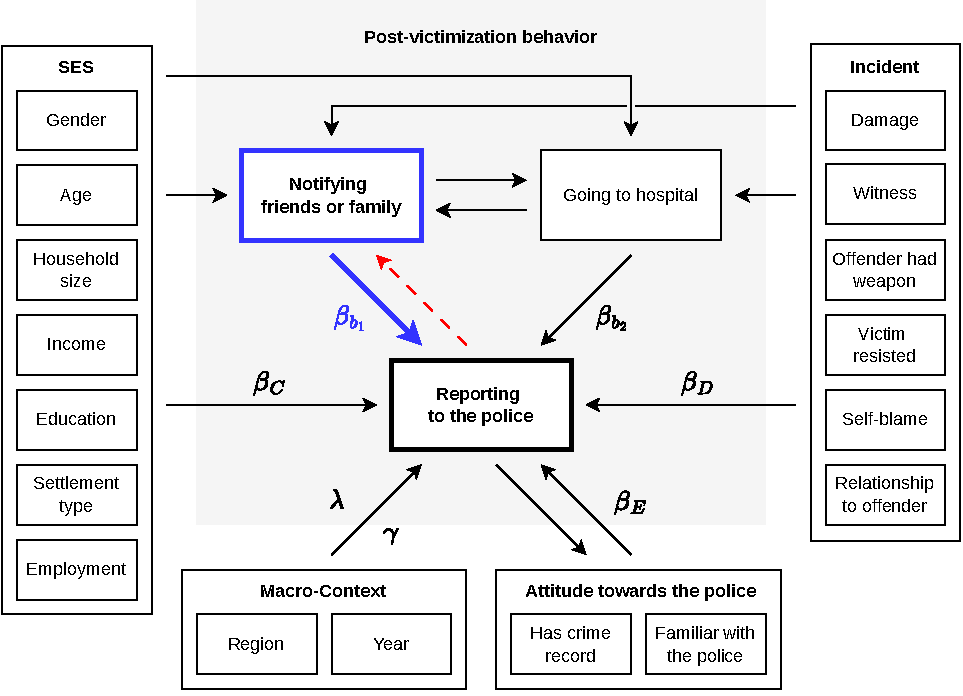
\includegraphics[width = 1\textwidth]{figures/causal_diagram_color.pdf}
		\caption{Causal diagram of decision making model}
		\label{fig:causal_diagram}	
	\end{figure}
	
	
	
	%Second, consider the situation from econometric perspective: after controlling for incident characteristics and other predictors common to both variables, there is no variation left in reporting variable that could explain variation in focus variable except for that which comes from the very act of communication with the police. In other words, the suspected endogeneity is possible only if we think that it is something in the experience with the law enforcement that prompts relation of the whole story to a friend or family. While not incomprehensible, this path seems less likely than the one in the opposite direction. Still, to reduce such possibility I estimate an additional model on a subset of data in which I remove observations where the police was notified but no case was initiated. The rationale: I assume that a popular scenario for \textit{incident---police---friends/family} path must be seeking help in police but being rejected and turning to intimate circle out of resentment for the perceived injustice. %Finally, I draw on the understanding that victims are more reluctant to cooperate with the police when offender is someone they know \citep{felson2016victims, gartner1995effect}: the denser the relationship between two parties the more averse a victim to introducing a third party into the relationship \citep{ruback1993comment}. This motivates my additional modeling on subset of cases where the offender was an intimate partner, friend, or relative: I can be more confident that in these cases a victim first turned to their intimate circle. Tables with regression results from additional models can be found in Appendices.
	%Second, this poses a problem only for a part of my argument. Indeed, although the existing literature suggests that the reverse order of these two events, \textit{reporting to the police $\rightarrow$ talking to friends or family}, must be rare there is still no way around the principal possibility that such cases are present in the data and introduce a positive bias in the estimation. 
	
	
	
	%This precludes causal inference regarding `counsellors' effect on reporting, allowing only associational conclusions.
	
	
	
	
	
	\begin{enumerate}[1.]
		\item Approval: a statement which confirms that all experimental protocols were approved by a named institutional and/or licensing committee. Please identify the approving body in the methods section
		
		\item Accordance: a statement explicitly saying that the methods were carried out in accordance with the relevant guidelines and regulations
		
		\item Informed consent (for experiments involving humans or human tissue samples): include a statement confirming that informed consent was obtained from all participants and/or their legal guardian/s
	\end{enumerate}
	
	If your manuscript includes potentially identifying patient/participant information, or if it describes human transplantation research, or if it reports results of a clinical trial then  additional information will be required. Please visit (\url{https://www.nature.com/nature-research/editorial-policies}) for Nature Portfolio journals, (\url{https://www.springer.com/gp/authors-editors/journal-author/journal-author-helpdesk/publishing-ethics/14214}) for Springer Nature journals, or (\url{https://www.biomedcentral.com/getpublished/editorial-policies\#ethics+and+consent}) for BMC.
	
	\section{Discussion}\label{sec12}
	
	Discussions should be brief and focused. In some disciplines use of Discussion or `Conclusion' is interchangeable. It is not mandatory to use both. Some journals prefer a section `Results and Discussion' followed by a section `Conclusion'. Please refer to Journal-level guidance for any specific requirements. 
	
	\section{Conclusion}\label{sec13}
	
	Conclusions may be used to restate your hypothesis or research question, restate your major findings, explain the relevance and the added value of your work, highlight any limitations of your study, describe future directions for research and recommendations. 
	
	In some disciplines use of Discussion or 'Conclusion' is interchangeable. It is not mandatory to use both. Please refer to Journal-level guidance for any specific requirements. 
	
	\backmatter
	
	\bmhead{Supplementary information}
	
	If your article has accompanying supplementary file/s please state so here. 
	
	Authors reporting data from electrophoretic gels and blots should supply the full unprocessed scans for key as part of their Supplementary information. This may be requested by the editorial team/s if it is missing.
	
	Please refer to Journal-level guidance for any specific requirements.
	
	\bmhead{Acknowledgements}
	
	Acknowledgements are not compulsory. Where included they should be brief. Grant or contribution numbers may be acknowledged.
	
	Please refer to Journal-level guidance for any specific requirements.
	
	\section*{Declarations}
	
	Some journals require declarations to be submitted in a standardised format. Please check the Instructions for Authors of the journal to which you are submitting to see if you need to complete this section. If yes, your manuscript must contain the following sections under the heading `Declarations':
	
	\begin{itemize}
		\item Funding
		\item Conflict of interest/Competing interests (check journal-specific guidelines for which heading to use)
		\item Ethics approval and consent to participate
		\item Consent for publication
		\item Data availability 
		\item Materials availability
		\item Code availability 
		\item Author contribution
	\end{itemize}
	
	\noindent
	If any of the sections are not relevant to your manuscript, please include the heading and write `Not applicable' for that section. 
	
	%%===================================================%%
	%% For presentation purpose, we have included        %%
	%% \bigskip command. Please ignore this.             %%
	%%===================================================%%
	\bigskip
	\begin{flushleft}%
		Editorial Policies for:
		
		\bigskip\noindent
		Springer journals and proceedings: \url{https://www.springer.com/gp/editorial-policies}
		
		\bigskip\noindent
		Nature Portfolio journals: \url{https://www.nature.com/nature-research/editorial-policies}
		
		\bigskip\noindent
		\textit{Scientific Reports}: \url{https://www.nature.com/srep/journal-policies/editorial-policies}
		
		\bigskip\noindent
		BMC journals: \url{https://www.biomedcentral.com/getpublished/editorial-policies}
	\end{flushleft}
	
	\begin{appendices}
		
		\section{Section title of first appendix}\label{secA1}
		
		An appendix contains supplementary information that is not an essential part of the text itself but which may be helpful in providing a more comprehensive understanding of the research problem or it is information that is too cumbersome to be included in the body of the paper.
		
		%%=============================================%%
		%% For submissions to Nature Portfolio Journals %%
		%% please use the heading ``Extended Data''.   %%
		%%=============================================%%
		
		%%=============================================================%%
		%% Sample for another appendix section			       %%
		%%=============================================================%%
		
		%% \section{Example of another appendix section}\label{secA2}%
		%% Appendices may be used for helpful, supporting or essential material that would otherwise 
		%% clutter, break up or be distracting to the text. Appendices can consist of sections, figures, 
		%% tables and equations etc.
		
	\end{appendices}
	
	%%===========================================================================================%%
	%% If you are submitting to one of the Nature Portfolio journals, using the eJP submission   %%
	%% system, please include the references within the manuscript file itself. You may do this  %%
	%% by copying the reference list from your .bbl file, paste it into the main manuscript .tex %%
	%% file, and delete the associated \verb+\bibliography+ commands.                            %%
	%%===========================================================================================%%
	
	\bibliography{bib}% common bib file
	%% if required, the content of .bbl file can be included here once bbl is generated
	%%\input sn-article.bbl
	
\end{document}
